\documentclass[11pt,a4paper]{article}
\usepackage[utf8]{inputenc}
\usepackage[T1]{fontenc}
\usepackage{amsfonts}
\usepackage[french]{babel}
\frenchbsetup{StandardLists=true}
\usepackage{enumitem}
\usepackage{amssymb}
\usepackage{amsmath}
\usepackage{parskip}
\usepackage[left=2cm,right=2cm,top=2cm,bottom=2cm]{geometry}
\usepackage{multirow}
\usepackage[dvipsnames]{xcolor}
\usepackage{fouriernc}
\usepackage{graphicx}
\usepackage{setspace}
\singlespacing
\usepackage{pstricks}
\usepackage{xkeyval}
\usepackage{pst-labo}
\usepackage{multicol}
\usepackage{caption}
\usepackage{fancyhdr}
\pagestyle{fancy}
\renewcommand\headrulewidth{1pt}
\fancyhead[L]{Lycée Denis Diderot}
\fancyhead[R]{Classe de Terminale}
\fancyfoot[C]{page \thepage}
\fancyfoot[R]{Année 2025 2026}
\fancyfoot[L]{Alexis RUIZ}
\usepackage{multirow,tabularx,booktabs}
\newcommand{\cadreblanc}[1]{%
\medskip\framebox[\linewidth][c]{%
\rule{0mm}{#1mm}}\par
\medskip}
\usepackage{awesomebox}
\setlength{\aweboxvskip}{0mm}
\usepackage{pifont}
\usepackage{chemmacros}
\usepackage{chemist}
\chemsetup{modules=all}
\renewcommand{\arraystretch}{2}
\newcommand*\acocher{\quitvmode{\fboxsep0pt \fboxrule0.8pt \fbox{\vrule height1.8ex depth.1ex width0pt \vrule height0pt depth0pt width1.9ex }}}
\newcommand*\cochevrai{\quitvmode{\fboxsep0pt \fboxrule0.8pt \fbox{\vrule height1.8ex depth.1ex width0pt \textcolor{BrickRed}{\ding{52}}\vrule height0pt depth0pt width0pt}}}
\usepackage{colortbl}

\definecolor{repcolor}{RGB}{180,0,0}
\newcommand{\rep}[1]{\textcolor{repcolor}{\textbf{#1}}}

\begin{document}

\begin{center}
\LARGE{\rep{CORRIGÉ} -- Evaluation -- Prévoir une réaction d'oxydo-réduction}\\[5mm]
\end{center}
\normalsize
\hrule
\vspace{8mm}

%=============================================================
\textbf{Exercice 1 : Cases à cocher}
%=============================================================

\ding{202} \textit{Indiquer pour chacune des affirmations si elle est vrai ou elle est fausse.}\\[0.3cm]

\renewcommand{\arraystretch}{1.5}
\begin{center}
\begin{tabularx}{15cm}{|p{11cm}|X|X|}
    \hline
    Affirmation & Vraie & Fausse\\
    \hline
    Une réaction d'oxydo-réduction est un échange de protons
        & & \cellcolor{BrickRed!20}\rep{$\boldsymbol{\times}$}\\
    \hline
    Une oxydation est une perte d'électrons
        & \cellcolor{BrickRed!20}\rep{$\boldsymbol{\times}$} & \\
    \hline
    Une réduction est un gain d'électrons
        & \cellcolor{BrickRed!20}\rep{$\boldsymbol{\times}$} & \\
    \hline
    Un oxydant perds des électrons
        & & \cellcolor{BrickRed!20}\rep{$\boldsymbol{\times}$}\\
    \hline
    Le métal cuivre est un réducteur
        & \cellcolor{BrickRed!20}\rep{$\boldsymbol{\times}$} & \\
    \hline
\end{tabularx}
\end{center}

\noindent\textcolor{BrickRed!70}{\small\textit{%
Remarques : Une réaction d'oxydo-réduction est un \textbf{transfert d'électrons} (et non de protons).
L'oxydant \textbf{gagne} des électrons (il se réduit). Le métal cuivre peut s'oxyder selon
\ch{Cu -> Cu\pch[2] + 2 e\mch[]}, c'est donc bien un réducteur.}}

\vfill

\ding{203} Les ions \ch{Cu\pch[2]} réagissent avec le métal zinc \ch{Zn}.\\[0.3cm]
\textbf{Réponses :}\\[0.3cm]
\renewcommand{\arraystretch}{1.5}
\begin{center}
\begin{tabularx}{13cm}{p{8.5cm}XX}
    L'ion \ch{Cu\pch[2]} est l'oxydant le plus fort
        & \cochevrai~~\rep{Oui} & \acocher~~Non \\
    L'ion \ch{Zn\pch[2]} est l'oxydant le plus fort
        & \acocher~~Oui & \cochevrai~~\rep{Non} \\
    Le métal cuivre est le réducteur le plus fort
        & \acocher~~Oui & \cochevrai~~\rep{Non} \\
    Le métal zinc est le réducteur le plus fort
        & \cochevrai~~\rep{Oui} & \acocher~~Non \\
\end{tabularx}
\end{center}

\noindent\textcolor{BrickRed!70}{\small\textit{%
La réaction a lieu donc \ch{Cu\pch[2]} est l'oxydant le plus fort (il reçoit les électrons de Zn),
et \ch{Zn} est le réducteur le plus fort (il cède ses électrons). Règle du $\gamma$.}}

\vfill

\ding{204} Les ions \ch{Cu\pch[2]} réagissent avec le métal fer \ch{Fe}. Équations exactes à cocher :\\[0.3cm]

\begin{multicols}{2}
    \cochevrai~~\rep{\ch{Cu\pch[2] + 2 e\mch[] -> Cu}} \\[3mm]
    \acocher~~\ch{Fe\pch[2] + 2 e\mch[] -> Fe} \\[3mm]
    \cochevrai~~\rep{\ch{Cu\pch[2] + Fe -> Cu + Fe\pch[2]}} \\[3mm]
    \acocher~~\ch{Cu -> Cu\pch[2] + 2 e\mch[]} \\[3mm]
    \cochevrai~~\rep{\ch{Fe -> Fe\pch[2] + 2 e\mch[]}} \\[3mm]
    \acocher~~\ch{Cu + Fe\pch[2] -> Cu\pch[2] + Fe} \\[3mm]
\end{multicols}

\noindent\textcolor{BrickRed!70}{\small\textit{%
Les trois équations correctes sont : la demi-équation de \textbf{réduction} de \ch{Cu\pch[2]},
la demi-équation d'\textbf{oxydation} de \ch{Fe}, et l'équation bilan.
La dernière équation (\ch{Cu + Fe\pch[2] ->}) représente la réaction inverse qui n'a pas lieu.}}

\vfill

\newpage

%=============================================================
\textbf{Exercice 2 : QCM} -- La bonne réponse est indiquée en \rep{rouge}.
%=============================================================

\begin{center}
\renewcommand{\arraystretch}{2.5}
\begin{tabular}{|>{\columncolor{Peach}}m{4mm}|p{4.5cm}||m{3.5cm}|m{3.5cm}|m{3.5cm}|}
    \hline
    \ding{202} & Au cours d'une réaction d'oxydo-réduction, l'oxydant
        & perd des protons
        & perd des électrons
        & \cellcolor{BrickRed!20}\rep{gagne des électrons} \\
    \hline
    \ding{203} & Dans quel cas l'ion en solution ne se dépose-t-il pas sur la lame métallique
        & ~~~~~~~~\raisebox{-.7\height}{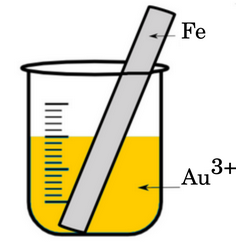
\includegraphics[scale=1]{images/QCm21.png}}
        & \cellcolor{BrickRed!20}~~~~~~~~\raisebox{-.7\height}{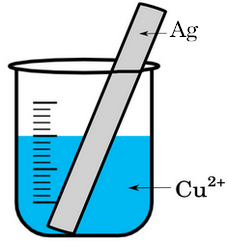
\includegraphics[scale=1.05]{images/QCm22.png}}\newline\rep{\ding{52}~Bonne réponse}
        & ~~~~~~~~\raisebox{-.7\height}{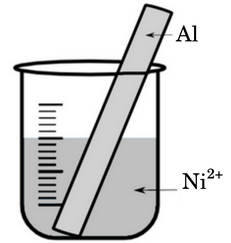
\includegraphics[scale=1]{images/QCm23.png}} \\
    \hline
    \ding{204} & Une réduction est
        & une perte d'électrons
        & \cellcolor{BrickRed!20}\rep{un gain d'électrons}
        & une perte de neutrons \\
    \hline
    \ding{205} & Au cours d'une réaction chimique l'ion Argent (\ch{Ag\pch[]}) se transforme en atome d'argent (\ch{Ag}), on dit
        & qu'il s'oxyde
        & qu'il se protège
        & \cellcolor{BrickRed!20}\rep{qu'il se réduit} \\
    \hline
    \ding{206} & Lors de la réduction des ions Cuivre ceux-ci
        & \cellcolor{BrickRed!20}\rep{gagnent deux \ch{e\mch[]}}
        & gagnent un \ch{e\mch[]}
        & perdent trois \ch{e\mch[]} \\
    \hline
    \ding{207} & Les ions chrome (\ch{Cr\pch[3]}) sont plus oxydants que les ions aluminium (\ch{Al\pch[3]}), quelle est l'équation possible
        & $\ch{Cr}+ \ch{Al\pch[3]}\longrightarrow \ch{Al} + \ch{Cr\pch[3]}$
        & $\ch{Al\pch[3]}+ \ch{Cr\pch[3]}\longrightarrow \ch{Al}+ \ch{Cr}$
        & \cellcolor{BrickRed!20}$\ch{Al} + \ch{Cr\pch[3]}\longrightarrow \ch{Cr}+ \ch{Al\pch[3]}$~\rep{\ding{52}} \\
    \hline
    \ding{208} & Que faut-il faire pour écrire l'équation bilan de $\ch{Al}\longrightarrow \ch{Al\pch[3]}+ 3\ch{e\mch[]}$ et $\ch{Zn\pch[2]}+2\ch{e\mch[]}\longrightarrow \ch{Zn}$
        & additionner membres à membres
        & multiplier par 3 la première demi-équation, multiplier par 2 la seconde, puis additionner
        & \cellcolor{BrickRed!20}\rep{multiplier par 2 la première demi-équation, multiplier par 3 la seconde, puis additionner} \\
    \hline
\end{tabular}
\end{center}

\vspace{3mm}
\noindent\textcolor{BrickRed!70}{\small\textit{%
Justifications : \ding{203}~\ch{Ag} dans \ch{Cu\pch[2]} : \ch{Cu\pch[2]/Cu} est moins oxydant que \ch{Ag\pch[]/Ag},
donc \ch{Cu\pch[2]} ne peut pas oxyder \ch{Ag} $\Rightarrow$ aucun dépôt.
\quad \ding{207}~Si \ch{Cr\pch[3]} plus oxydant, alors \ch{Cr\pch[3]} oxyde \ch{Al} : \ch{Al + Cr\pch[3] -> Cr + Al\pch[3]}.
\quad \ding{208}~PPCM(3,2)~=~6 : $\times 2$ la 1\textsuperscript{re}, $\times 3$ la 2\textsuperscript{e}, ce qui donne
$2\,\ch{Al} + 3\,\ch{Zn\pch[2]} \longrightarrow 2\,\ch{Al\pch[3]} + 3\,\ch{Zn}$.}}

\newpage

%=============================================================
\textbf{Exercice 3 : Béchers}
%=============================================================

\vspace{3mm}

\textbf{Exp~~\ding{202} :} Grenaille d'argent (\ch{Ag}) dans une solution d'ions cuivre (\ch{Cu\pch[2]})

\medskip
\noindent La réaction a-t-elle lieu ?~~ $\Box$~oui \quad \fbox{\rep{non}} \\[2mm]
\rep{La réaction \textbf{n'a pas lieu}.}\\[1mm]
\textcolor{BrickRed!70}{\small\textit{Justification : D'après la classification des oxydoréducteurs,
\ch{Ag\pch[]/Ag} est plus oxydant que \ch{Cu\pch[2]/Cu}
(les ions \ch{Ag\pch[]} sont de meilleurs oxydants que \ch{Cu\pch[2]}).
Par conséquent, \ch{Cu\pch[2]} \textbf{ne peut pas} oxyder le métal \ch{Ag}.
Aucun dépôt ne se forme.}}

\vspace{8mm}

\textbf{Exp~~\ding{203} :} Grenaille de zinc (\ch{Zn}) dans une solution d'ions platine (\ch{Pt\pch[2]})

\medskip
\noindent La réaction a-t-elle lieu ?~~ \fbox{\rep{oui}} \quad $\Box$~non \\[2mm]
\rep{La réaction \textbf{a lieu} : \ch{Pt\pch[2]} est plus oxydant que \ch{Zn\pch[2]}.}\\[3mm]
Demi-équations :\\[1mm]
\begin{tabular}{ll}
Réduction (oxydant \ch{Pt\pch[2]}) : & \rep{\ch{Pt\pch[2] + 2 e\mch[] -> Pt}} \\
Oxydation (réducteur \ch{Zn}) :      & \rep{\ch{Zn -> Zn\pch[2] + 2 e\mch[]}} \\
\end{tabular}\\[3mm]
Équation de réaction (les électrons s'annulent directement, même nombre) :\\[1mm]
\hspace{1cm}\rep{\ch{Pt\pch[2] + Zn -> Pt + Zn\pch[2]}}

\vspace{8mm}

\textbf{Exp~~\ding{204} :} Grenaille d'aluminium (\ch{Al}) dans une solution d'ions étain (\ch{Sn\pch[2]})

\medskip
\noindent La réaction a-t-elle lieu ?~~ \fbox{\rep{oui}} \quad $\Box$~non \\[2mm]
\rep{La réaction \textbf{a lieu} : \ch{Sn\pch[2]} est plus oxydant que \ch{Al\pch[3]}.}\\[3mm]
Demi-équations :\\[1mm]
\begin{tabular}{ll}
Réduction (\ch{Sn\pch[2]}) : & \rep{\ch{Sn\pch[2] + 2 e\mch[] -> Sn}} \quad $(\times 3)$ \\
Oxydation (\ch{Al}) :         & \rep{\ch{Al -> Al\pch[3] + 3 e\mch[]}} \quad $(\times 2)$ \\
\end{tabular}\\[3mm]
Équation de réaction (PPCM(2,3)~=~6, on multiplie la 1\textsuperscript{re} par 3, la 2\textsuperscript{e} par 2) :\\[1mm]
\hspace{1cm}\rep{$3\,\ch{Sn\pch[2]} + 2\,\ch{Al} \longrightarrow 3\,\ch{Sn} + 2\,\ch{Al\pch[3]}$}

\vspace{8mm}

\textbf{Exp~~\ding{205} :} Grenaille de magnésium (\ch{Mg}) dans une solution d'ions fer (\ch{Fe\pch[2]})

\medskip
\noindent La réaction a-t-elle lieu ?~~ \fbox{\rep{oui}} \quad $\Box$~non \\[2mm]
\rep{La réaction \textbf{a lieu} : \ch{Fe\pch[2]} est plus oxydant que \ch{Mg\pch[2]}.}\\[3mm]
Demi-équations :\\[1mm]
\begin{tabular}{ll}
Réduction (\ch{Fe\pch[2]}) : & \rep{\ch{Fe\pch[2] + 2 e\mch[] -> Fe}} \\
Oxydation (\ch{Mg}) :         & \rep{\ch{Mg -> Mg\pch[2] + 2 e\mch[]}} \\
\end{tabular}\\[3mm]
Équation de réaction (les électrons s'annulent directement) :\\[1mm]
\hspace{1cm}\rep{\ch{Fe\pch[2] + Mg -> Fe + Mg\pch[2]}}

\end{document}
